\chapter{Neutrino Physics}
\label{chap:theory}
This chapter introduces the experimental evidence for the neutrino and neutrino oscillations, outlines the theory of neutrino oscillations, and discusses neutrino interactions in the $E_\nu\sim1-10 \text{ GeV}$ range, relevant to long baseline neutrino oscillation experiments.

\section{The Discoveries of the Neutrinos}
Neutrinos were initially proposed as a solution to the apparent violation of the conservation of four-and angular momentum in James Chadwick's measurements of beta decay in 1932\cite{Chadwick1,Chadwick2}. Inspired by Wolfgang Pauli's new elementary particle ``the neutron''\footnote{Which had characteristics of what we today call a nucleon and a neutrino}\cite{pauli_1933}, Enrico Fermi built his theory of $\beta$-decay\cite{fermi_1934}, in which the observable process $n \rightarrow p + e^-$ is always accompanied by an invisible four-momentum carrier, the electron anti-neutrino.

The neutrino remained elusive until Reines and Cowan in 1953 devised their experiments using the inverse beta decay (IBD) process, $\bar{\nu}_e + p \rightarrow n + e^+$, near a nuclear reactor\cite{reines_cowan_1,reines_cowan_2}. The experiment consisted of two tanks of water sandwiched by three liquid scintillator tanks with photo multiplier tubes (PMTs). The water was doped with 40 kg $\text{CdCl}_2$, which could detect free neutrons through capture. The electron anti-neutrinos were emitted by the nuclear reactor, interacted with the protons in the water, producing a prompt signal from $e^+ + e^- \rightarrow 2\gamma$. The free neutron was detected $\sim5\mu\text{s}$ after the prompt $2\gamma$ from $n + ^{108}\text{Cd} \rightarrow ^{109m}\text{Cd} \rightarrow ^{109}\text{Cd} + \gamma$. The experiment also took data from a reactor off period, demonstrating a significant reduction in neutrino event rates. Modern reactor neutrino oscillation experiments such as Daya Bay\cite{daya_bay} operate much on the same principle. The experiment was complemented by measurements by R. Davis  in 1964\cite{davis}, which exposed tanks of $^{37}\text{Cl}$ to reactor electron anti-neutrinos, interacting through $\bar{\nu}_e + ^{37}\text{Cl} \rightarrow e^- + ^{37}\text{Ar}$, which would violate lepton number conservation. The experiment found no excess of $^{37}\text{Ar}$, and instead set limits on the solar neutrino flux. 

The field quickly developed after the first measurements and in 1962 Lederman, Schwartz, Steinberger and others\cite{lederman} observed another flavour of neutrino, the muon neutrino. They used a beam of protons impinging a target, creating a $\pi$ dominated beam which decayed following $\pi^+ \rightarrow \mu^+ + \nu_\mu$, and looked for subsequent interactions of the $\nu_\mu$ in a 10 tonne shielded aluminium spark chamber. The experiment was later confirmed by measurements at CERN in 1964\cite{cern_spark,cern_spark2}.

When the third charged lepton, the $\tau$, was discovered at SLAC's $e^+e^-$ accelerator in 1975\cite{tau_disc}, the search for its neutrino partner started. Its existence was already hinted at in $\tau$ decays and was discovered at DONUT in 2000\cite{tau_nu_disc}. The discovery of the $\nu_\tau$ and the three neutrino flavours was largely expected from precise measurements of $Z$ decays at the Large Electron Positron (LEP) and the Stanford Linear Accelerator (SLAC), which found the number of active neutrino flavours, assuming the Standard Model, as $N_\nu = 2.9840\pm0.0082$\cite{lep}. This has also been confirmed by cosmological data from Planck and others, $N_\text{eff} = 3.04\pm0.18$\footnote{$N_\text{eff}=3.0\pm0.4$ and $\sum m_\nu < 0.22 \text{ eV}$ when varying both $N_\text{eff}$ and $\sum m_\nu$.}\cite{planck}.

\section{Neutrino Oscillations}
\label{sec:theory:osc}
The discovery of neutrino oscillations, detailed in \autoref{sec:exp_overview}, is a direct consequence of neutrino mass. B. Pontecorvo\cite{p1,p2,pontecorvo_gribov}, Z. Maki, M. Nakagawa and S. Sakata\cite{mns} developed the PMNS formalism, widely used by the oscillation community today. This section highlights some crucial components of the theory and how it has been applied in the field.

The PMNS formalism starts by introducing a neutrino mass eigenstate $\ket{\nu_i}$, which is a linear superposition of the flavour eigenstates participating in the weak interaction $\ket{\nu_\alpha}$ with $n$ neutrino states,
\begin{equation}
\ket{\nu_i} = \sum_\alpha^n U_{\alpha i} \ket{\nu_\alpha}
\end{equation}
where the unitary matrix $U$ is generally expressed as
\begin{equation}
U = 
\begin{pmatrix}
	U_{e 1} & U_{e 2} & U_{e 3} \\
	U_{\mu 1} & U_{\mu 2} & U_{\mu 3} \\
	U_{\tau 1} & U_{\tau 2} & U_{\tau 3} \\
\end{pmatrix}
\end{equation}
This echoes that of quark mixing proposed by Cabbibo\cite{cabbibo}, Kobayashi and Maskawa\cite{km}. The superposition leads to a probability of observing neutrino flavour change from flavour $\alpha$ to $\beta$ over distance $L$ for a neutrino with energy $E$ in which the square of two neutrino mass states are separated by $\Delta^2 m_{ij} = m^2_i - m^2_j$,
\begin{equation}
P(\nu_\alpha \rightarrow \nu_\beta) = |\braket{\nu_\beta|\nu_\alpha(t)}|^2 = \sum_{k,j} U*_{\alpha k} U_{\beta k} U*_{\alpha j} U_{\beta j} \exp{ \left( -i\frac{\Delta m^2_{i j} L}{2E} \right)}
\end{equation}

Then using the squared unitarity relation we finally get\cite{boris_mixing},
\begin{align}
P(\nu_\alpha \rightarrow \nu_\beta) = \delta_{\alpha \beta} &- 4\sum_{i>j} Re\left(U^*_{\alpha i} U_{\beta i} U_{\alpha j} U^*_{\beta j}\right)  \sin^2 ( \Delta m^2_{ij}\frac{L}{4E} ) \\
									&+(-) 2\sum_{i>j} Im\left( U^*_{\alpha i} U_{\beta i} U_{\alpha j} U^*_{\beta j} \right) \sin ( \Delta m^2_{ij}\frac{L}{2E} )
\end{align}
where the negative sign is picked up for anti-neutrinos.

The PMNS matrix is often parameterised into three separate matrices with their own mixing angles $\theta_{13},\theta_{23}$ and $\theta_{12}$ and a complex phase $\delta$, where $c_{ij}=\cos\theta_{ij}$ and $s_{ij}=\sin\theta_{ij}$\cite{boris_mixing},
\begin{equation}
U = 
\begin{pmatrix}
1 & 0 & 0 \\
0 & c_{23} & s_{23} \\
0 & -s_{23} & c_{23} \\
\end{pmatrix}
\begin{pmatrix}
c_{13} & 0 & s_{13}e^{-i\delta} \\
0 & 1 & 0 \\
-s_{13}e^{-i\delta} & 0 & c_{13} \\
\end{pmatrix}
\begin{pmatrix}
c_{12} & s_{12} & 0 \\
-s_{12} & c_{12} & 0 \\
0 & 0 & 1 \\
\end{pmatrix}
\end{equation}
where the $(1,2)$ parameters are referred to as ``solar'', $(2,3)$ as ``atmospheric'', and $(1,3)$ as ``reactor''. The $\delta$ is commonly referred to as the CP violating Dirac phase, $\delta_{CP}$. 

Reducing down to two neutrino mass states (where the third is degenerate with another), we obtain to a simpler mixing matrix $U$,
\begin{equation}
U = 
\begin{pmatrix}
\cos\theta & \sin\theta \\
- \sin\theta & \cos \theta \\
\end{pmatrix}
\end{equation}
and an oscillation probability of
\begin{equation}
P(\nu_\alpha \rightarrow \nu_\beta) = \delta_{\alpha \beta} -(+) \sin^2 \left( 2\theta \right) \sin^2 \left( \frac{1.267 \Delta m^2 \left[\text{eV}^2\right] L\left[\text{km}\right]}{E\left[\text{GeV}\right]} \right)
\label{eq:two_flavour}
\end{equation}
where the positive sign is picked up when $\beta = \alpha$. The sinusoidal oscillation of the neutrino flavour states is clear in \autoref{eq:two_flavour}, whose period is controlled by the parameter $\Delta m^2$ and amplitude by the mixing angle $\theta$. The maximum probability to observe oscillation for a fixed mixing angle is $L/E \sim 1.25/\Delta m^2$ which for $\Delta m^2 \sim 2.5\times10^{-3}\text{ eV}^2$ and $L\sim300\text{ km}$ means $E=0.6\text{ GeV}$, placing an experiment like T2K ($L=295\text{ km}, E = 0.6\text{ GeV}$) near maximum.

The final ingredient in the oscillation probability is to account for effects from traversing matter rather than vacuum, often referred to as the Mikheyev-Smirnov-Wolfenstein (MSW) effect\cite{barger,parke,wolfenstein,msw}. The effect sets electron neutrinos apart from muon and tau neutrinos, since they have an additional weak interaction with electrons in matter, shown in \autoref{fig:msw_effect}.
\begin{figure}[h]
	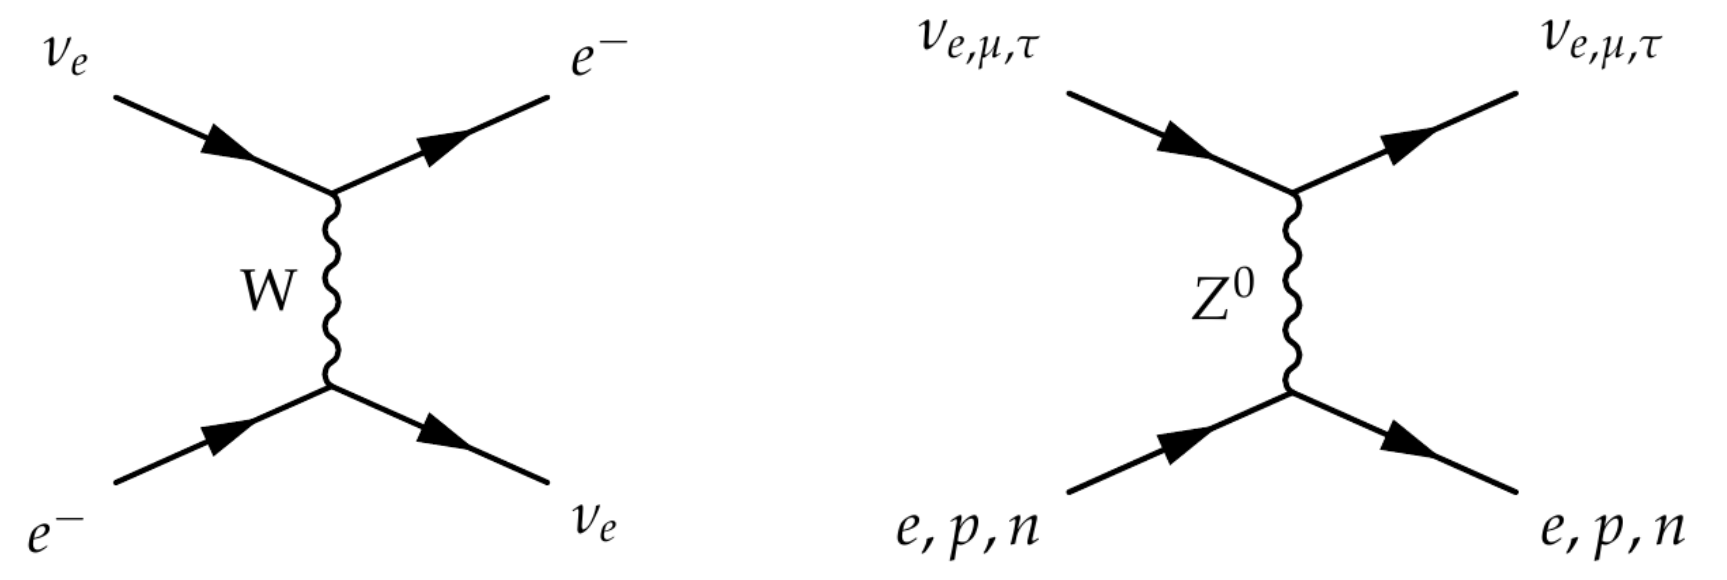
\includegraphics[width=0.8\textwidth, trim={0mm 0mm 0mm 0mm}, clip,page=1]{figures/theory/msw_effect}
	\caption{Interaction diagrams with matter for different neutrino flavours}
	\label{fig:msw_effect}
\end{figure}

Electron neutrinos experience a modified Hamiltoninan potential $\Delta V = 2\sqrt{2}G_F E_\nu N_e$, where $G_F$ is the Fermi constant, $E_\nu$ is the neutrino energy and $N_e$ is the electron number density of the matter. The effect modifies the oscillation probability to have dependence on $\sin^2 \Delta m^2$ and $\sin \Delta m^2$, inferring the sign of $\Delta m^2$ can be resolved when significant matter interactions occur\cite{msw_summary}.

\section{Neutrino Interactions}
\label{sec:theory:int}
Neutrino-matter interactions are a dominant systematic for current long-baseline, intermediate energy neutrino oscillation experiments. Their parameterisation for this analysis is given in \autoref{subsec:syst_xsec}, with an overview provided here. Detailed discussions can be found in \cite{katori_martini,ulrich_review,nieves_review}.

Generally, the $E_\nu \sim 1-10\text{ GeV}$ regime is referred to as the ```intermediate energy region'''. At the low end, nuclear effects such as nucleon-nucleon correlations\cite{nieves1,nieves2}, $\Delta$ in-medium corrections\cite{nuclear_effects_1pi} and nucleus spectral functions \cite{benhar} are important, whereas the high-end is dominated by deep inelastic scattering (DIS). The transition regions between producing no, single and multiple pions is particularly poorly modelled. Neutrino-nucleus and nucleon scattering theory is often inspired by results from electron scattering\cite{joanna}, such as CLAS\cite{clas} at JLAB. The experiments have the benefit of a narrow beam energy window, and so can study nuclear effects at specific $Q=P_{in}-P_{out}$ to the nucleus. 

In Monte Carlo event generators, the neutrino interaction process is commonly factorised into four parts: 1) A nucleon is simulated from a nuclear model and is used as a target for the neutrino interaction and we boost into its rest-frame, 2) The neutrino interacts with chosen nucleon which is now at rest, equivalent to a neutrino-nucleon interaction, 3) The outgoing particles from the fundamental vertex are propagated through the nucleus with radiative and final state interactions applied, 4) The particles are boosted back into the lab frame.

The total cross-sections in $E_\nu$, $\sigma(E_\nu)$, for the NEUT 5.3.3\cite{neut} generator used by T2K are shown in \autoref{fig:neut_xsecs}. At T2K energies ($E_\nu\sim0.6\text{ GeV}$) the primary interaction mode is CCQE. Charged pion production becomes important at $E_\nu\sim1\text{ GeV}$, and multi-$\pi$ and DIS above $E_\nu\sim2.5\text{ GeV}$. Since this analysis aims to minimise systematics for oscillation analyses---which select the charged-current 0$\pi$ final state at SK---the 0$\pi$ systematics have the largest impact.
\begin{figure}[h]
	\centering
	\begin{subfigure}[t]{0.42\textwidth}
		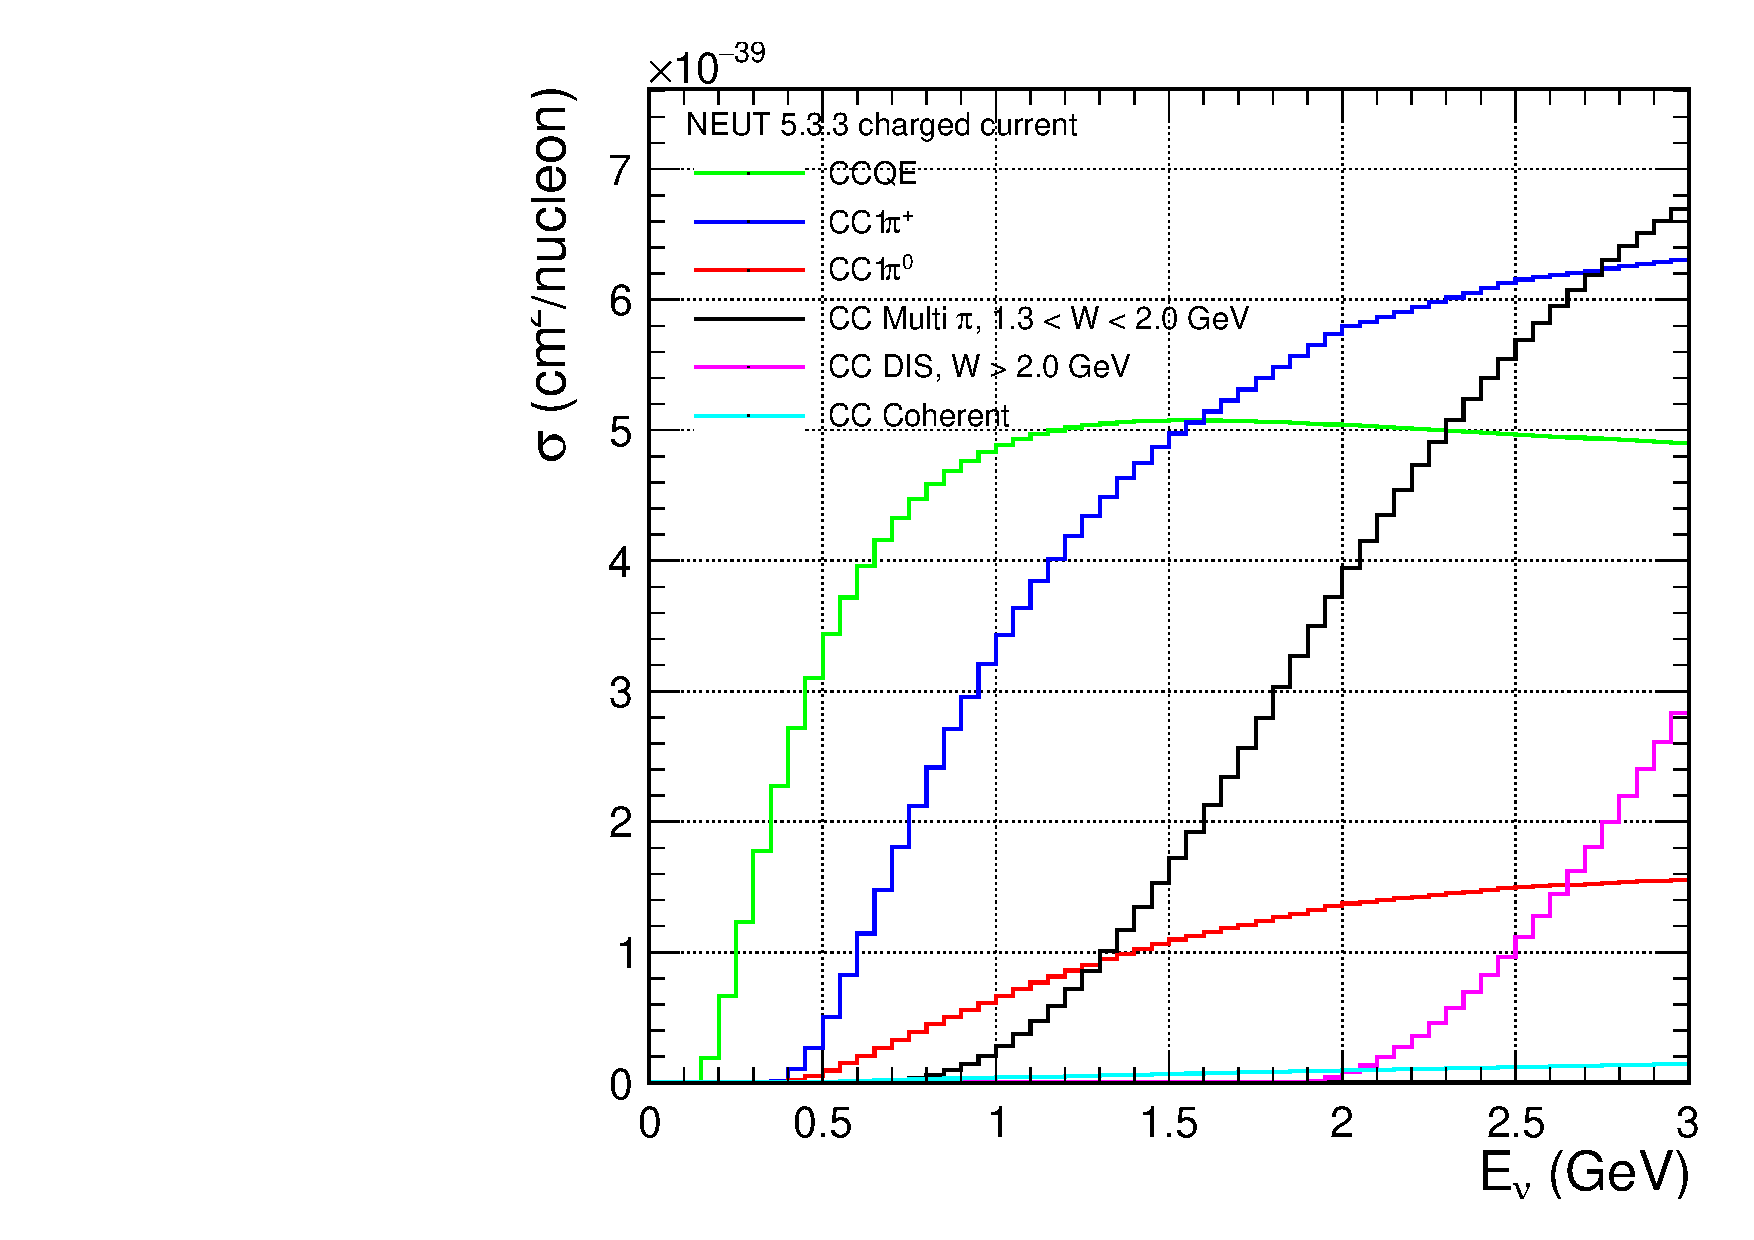
\includegraphics[width=\textwidth, trim={0mm 0mm 0mm 0mm}, clip,page=1]{figures/niwg/NEUT_533_xsecs}
		\caption{Charged current}
	\end{subfigure}
	\begin{subfigure}[t]{0.42\textwidth}
		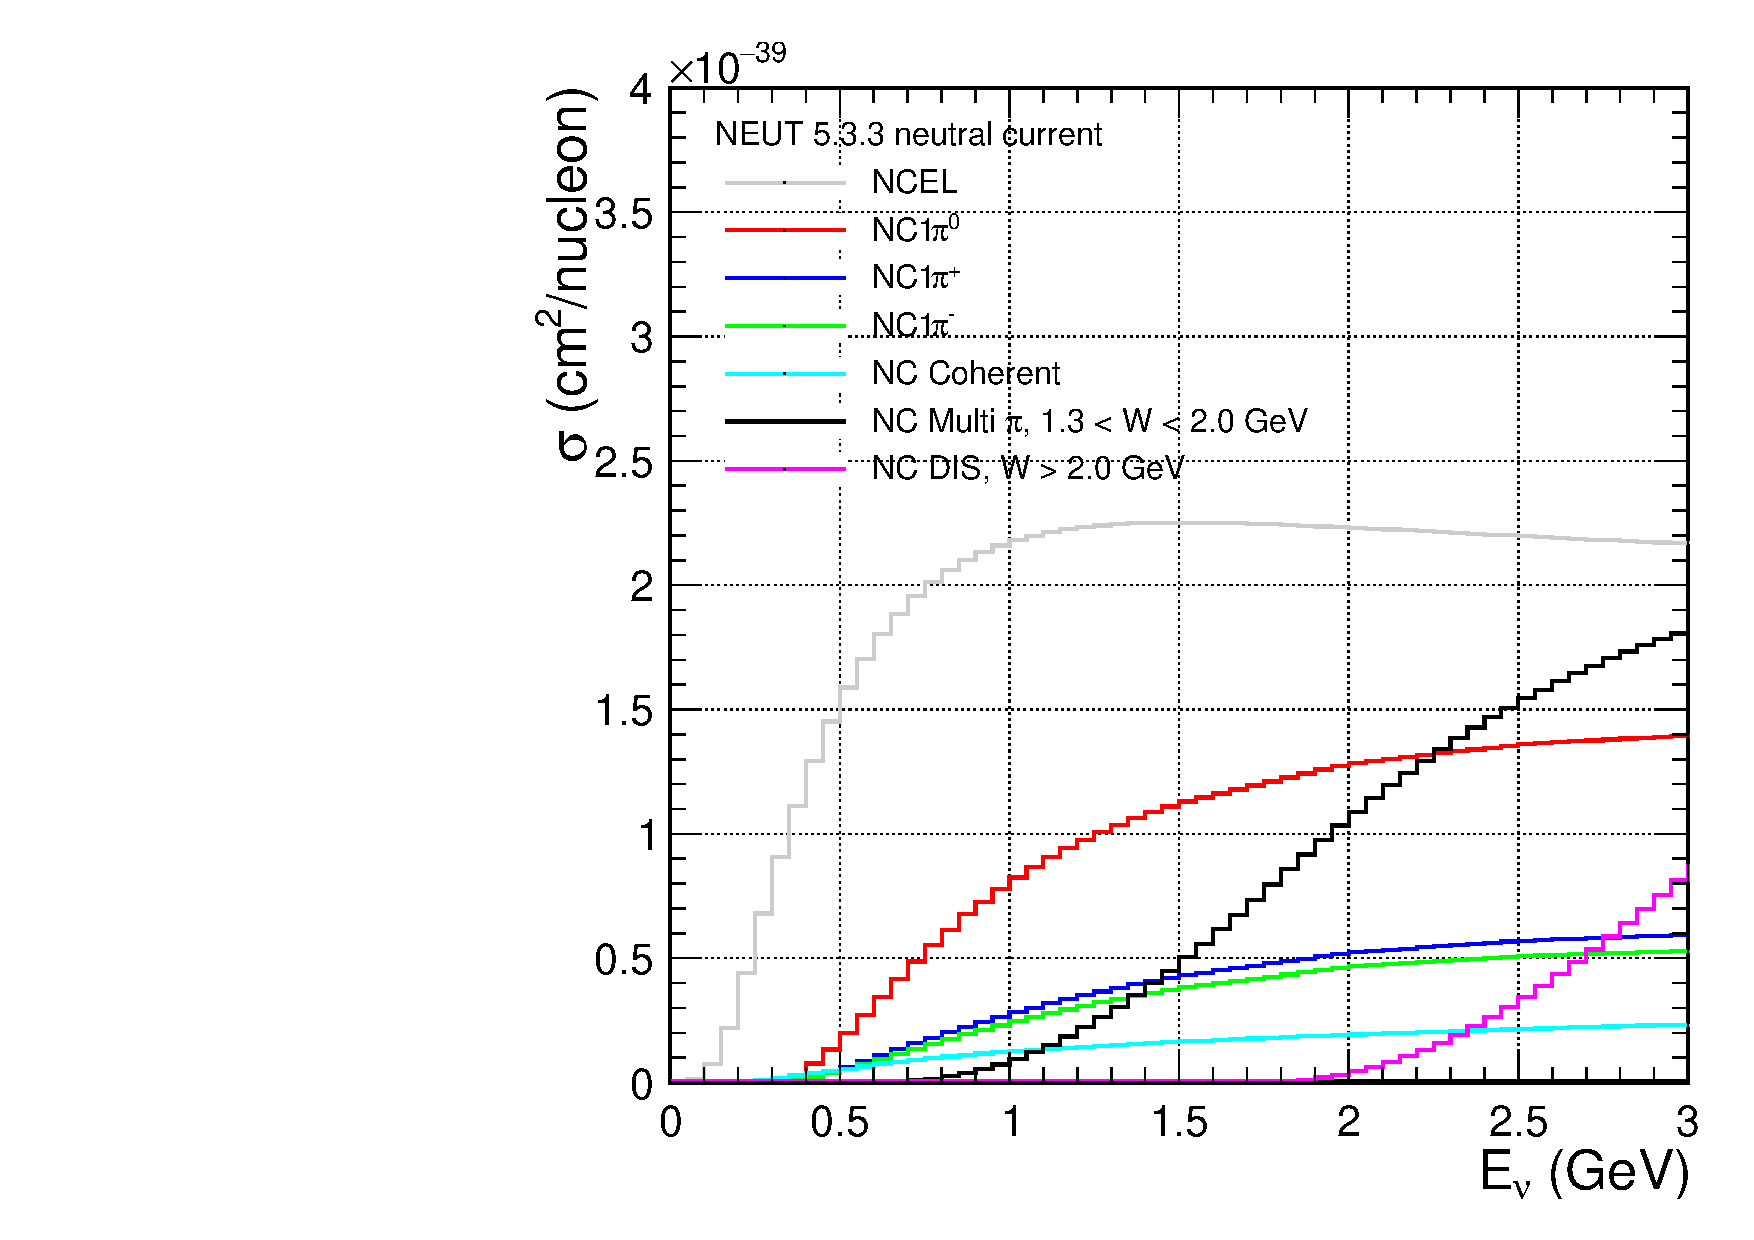
\includegraphics[width=\textwidth, trim={0mm 0mm 0mm 0mm}, clip,page=1]{figures/niwg/NEUT_533_xsecs_NC}
		\caption{Neutral current}
	\end{subfigure}
	\caption{Total cross-sections from the NEUT 5.3.3\cite{neut} neutrino interaction generator}
	\label{fig:neut_xsecs}
\end{figure}

\subsection{CC0$\pi$}
\autoref{fig:cc0pi_diag} shows some pseudo diagrams of the definition of the 0$\pi$, CCQE and one 2p2h process. The CC0$\pi$ signal definition does not include hadronic information, so the CCQE and 2p2h processes both produce 0$\pi$ final states. T2K uses the CCQE diagram for neutrino energy reconstruction, assuming a nucleon at rest. If 2p2h events are included in the selection it biases $E_\nu$, and wrongly estimating the bias has a noticeable effect on oscillation parameters. The same holds true for including single pion events due to unreconstructed pions or final state interactions.
\begin{figure}[h]
	\centering
	\begin{subfigure}[t]{0.32\textwidth}
		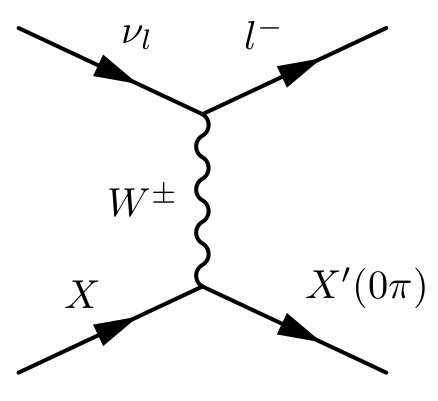
\includegraphics[width=\textwidth, trim={0mm 0mm 0mm 0mm}, clip,page=1]{figures/niwg/diagrams/CC0pi}
		\caption{CC0$\pi$}
	\end{subfigure}
	\begin{subfigure}[t]{0.32\textwidth}
		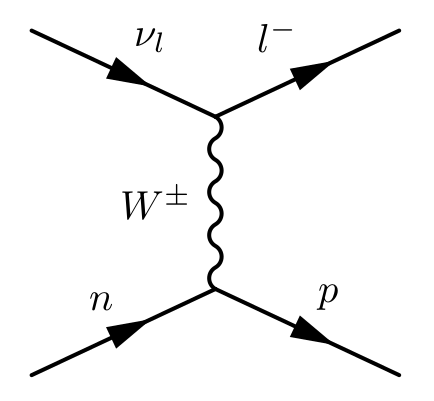
\includegraphics[width=\textwidth, trim={0mm 0mm 0mm 0mm}, clip,page=1]{figures/niwg/diagrams/CCQE}
		\caption{CCQE}
	\end{subfigure}
	\begin{subfigure}[t]{0.32\textwidth}
		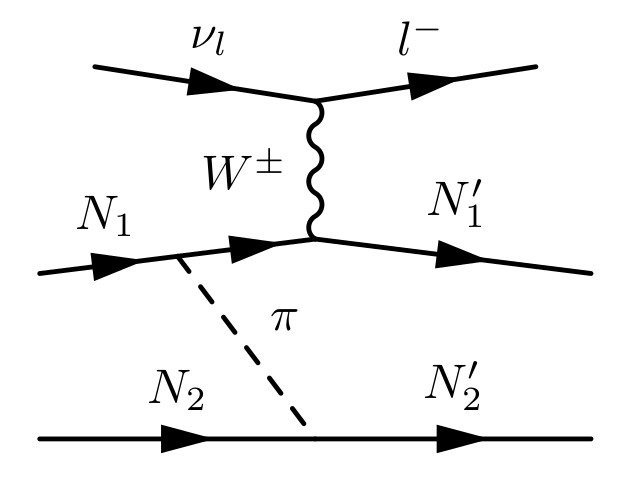
\includegraphics[width=\textwidth, trim={0mm 0mm 0mm 0mm}, clip,page=1]{figures/niwg/diagrams/2p2h_possibly}
		\caption{A 2p2h process}
	\end{subfigure}
	\caption{CC0$\pi$, CCQE and 2p2h pseudo-diagrams}
	\label{fig:cc0pi_diag}
\end{figure}

Generally, the neutrino-nucleon CCQE interaction is relatively well understood. The current effort in the field is to understand the impact of form factor choices, numerous nuclear effects, and minimising the models' impacts on cross-section and oscillation measurements.

\subsection{Single Pion Production}
\autoref{fig:1pi_diags} shows the dominant charged-current neutrino-nucleon interactions giving rise to single pion production (SPP). The interaction proceeds by a resonant state here labelled as $\Delta$, which is dominant at T2K energies. SPP makes up $\sim20\%$ of selected 0$\pi$ events at SK due to missing pions.
\begin{figure}[h]
	\centering
	\begin{subfigure}[t]{0.32\textwidth}
		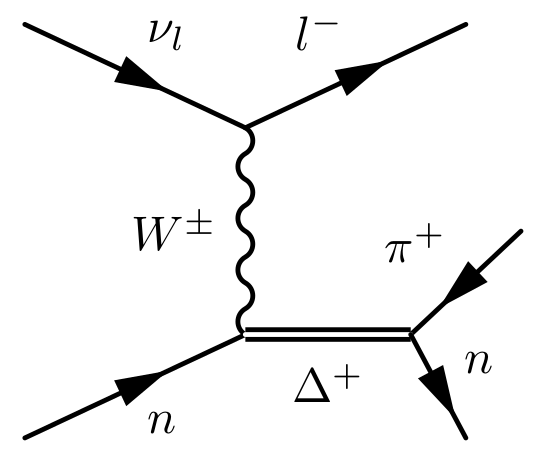
\includegraphics[width=\textwidth, trim={0mm 0mm 0mm 0mm}, clip,page=1]{figures/niwg/diagrams/CC1npip}
		\caption{CC1$\pi^+$1n}
	\end{subfigure}
	\begin{subfigure}[t]{0.32\textwidth}
		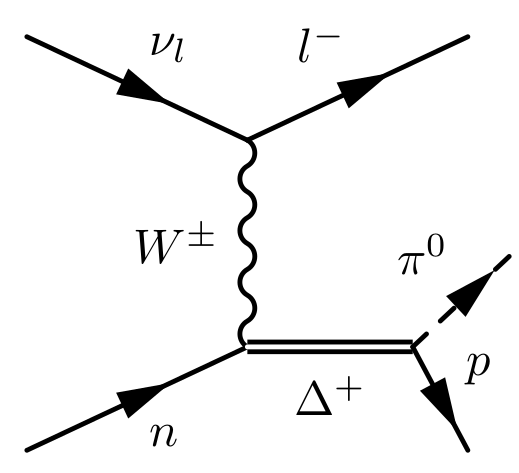
\includegraphics[width=\textwidth, trim={0mm 0mm 0mm 0mm}, clip,page=1]{figures/niwg/diagrams/CC1pi0}
		\caption{CC1$\pi^0$}
	\end{subfigure}
	\begin{subfigure}[t]{0.32\textwidth}
		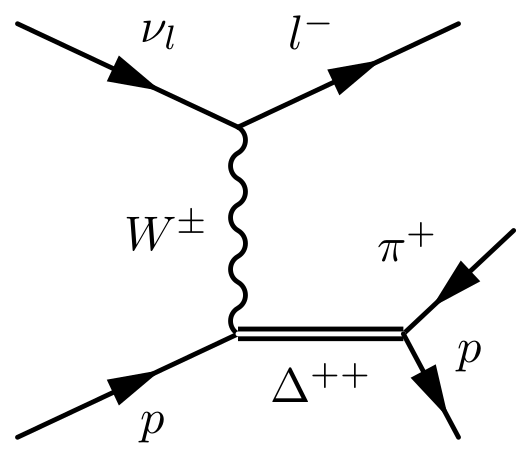
\includegraphics[width=\textwidth, trim={0mm 0mm 0mm 0mm}, clip,page=1]{figures/niwg/diagrams/CC1ppip}
		\caption{CC1$\pi^+$1p}
	\end{subfigure}
	\caption{Charged-current single pion production on a nucleon via a $\Delta$ resonances}
	\label{fig:1pi_diags}
\end{figure}

Contrary to the CCQE interaction, single pion production on free nucleons is poorly modelled. The low hadronic mass $(W)$ regime where the single $I_{3/2}$ $\Delta^{++}\rightarrow p+\pi^+$ interaction dominates can be considered understood, although resonance-resonance and resonance-non-resonance interference present at higher $W$ is not. Additionally, in-medium effects from resonance fields propagating the nucleus are poorly understood and multi-nucleon couplings often unmodelled\cite{nustec,katori_martini}.

\subsection{Multi-$\pi$ and DIS}
The transition from SPP to DIS is generally referred to soft inelastic scattering (SIS). NEUT uses a custom interpolation between $1.3 < W < 2.0$, selecting events with $N_\pi>1$ to avoid double counting SPP cross-sections. Other generators such as GENIE\cite{genie} and NuWro\cite{NuWro} use different implementations. A pseudo diagram is shown in \autoref{fig:dis_diags}, where fragmentation causes the pion emissions.

\subsection{Subdominant Interactions}
Subdominant interactions with small interaction cross-sections can populate very specific signal regions, e.g. NC$1\gamma$ and NC1$\pi^0$ mimicking $\nu_e + X\rightarrow e^- + X'$, and differences in $\nu_e$ vs $\nu_\mu$. Historically, there is much less cross-section data on NC interactions than CC and barely any using electron neutrinos, and it is common to trust model extrapolation from CC to NC rather than test against data. 

The charged current coherent process shown in \autoref{fig:coh_diags} occupies a very specific phase space: the very forward going, collinear lepton-pion, low $Q^2$ region. This is important since it has the same final state as single pion production, although not produced through a resonance, making up about 10\% of the most forward-going \cosmu bin in CC1$\pi$ selections.
\begin{figure}[h]
	\centering
	\begin{subfigure}[t]{0.42\textwidth}
		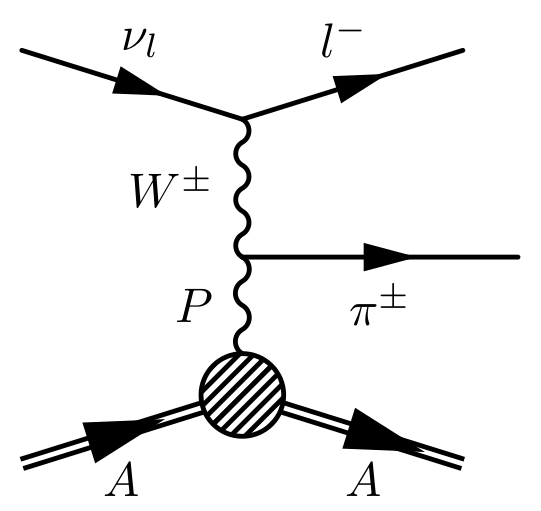
\includegraphics[width=\textwidth, trim={0mm 0mm 0mm 0mm}, clip,page=1]{figures/niwg/diagrams/CCcoh}
		\caption{CC coherent}
		\label{fig:coh_diags}
	\end{subfigure}
	\begin{subfigure}[t]{0.42\textwidth}
		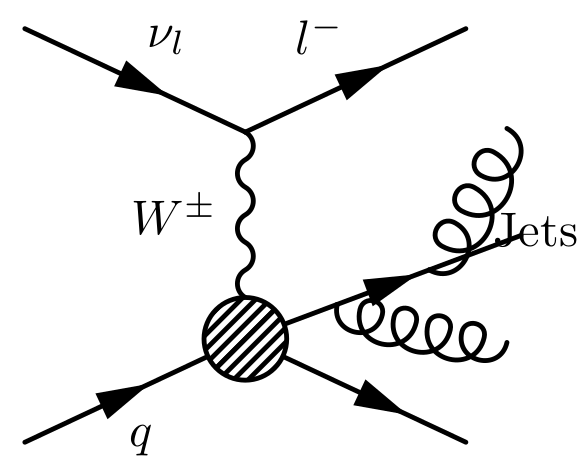
\includegraphics[width=\textwidth, trim={0mm 0mm 0mm 0mm}, clip,page=1]{figures/niwg/diagrams/CCmultipion}
		\caption{CC DIS}
		\label{fig:dis_diags}
	\end{subfigure}
	\caption{Coherent and multi-pion/DIS scattering diagrams}
	\label{fig:coh_dis_diags}
\end{figure}

\subsection{Intranuclear Hadronic Cascades}
The nuclear cascade following the initial neutrino-nucleon interaction is often handled by a microscopic hadron propagation, in which interaction probabilities in the nucleus are calculated for positions in the nucleus, seen in \autoref{fig:fsi_cascade}. 

Simulations can be considered to agree relatively well with pion scattering data\cite{thesis_elder}, but there are concerns that extrapolating results into the neutrino-nucleus interaction is unjustifiable\cite{ulrich_review}. More realistic models exist in the Giessen-Boltzmann-Uehling-Uhlenbeck (GiBUU)\cite{gibuu} generator, although its role as a primary generator in neutrino physics is currently not viable due to computational requirements.
\begin{figure}[h]
	\centering
	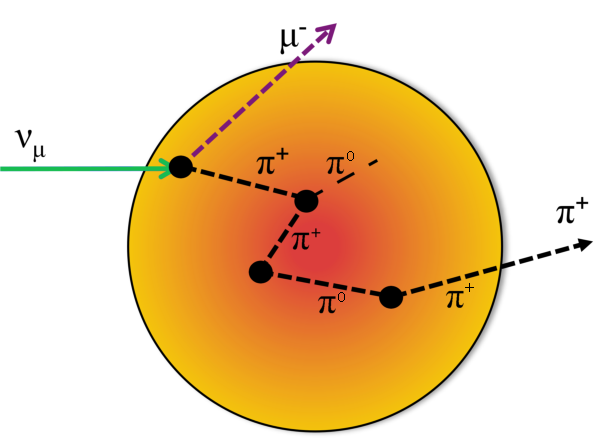
\includegraphics[width=0.3\textwidth, trim={0mm 0mm 0mm 0mm}, clip,page=1]{figures/niwg/diagrams/cascade}
	\caption{An example of a pion FSI cascade}
	\label{fig:fsi_cascade}
\end{figure}

\section{Experimental Overview}
\label{sec:exp_overview}
Neutrino oscillations is now an established physics phenomena, cemented by awarding the 2015 Nobel Prize in Physics to Kajita-san (spokesperson for SK) and Art McDonald (spokesperson for SNO) for their experiments' measurements of solar and atmospheric neutrino oscillations. This section gives a brief introduction and overview of neutrino oscillation experiments and production mechanisms, summarised in \autoref{fig:all_neutrino_expts}.
\begin{figure}[h]
	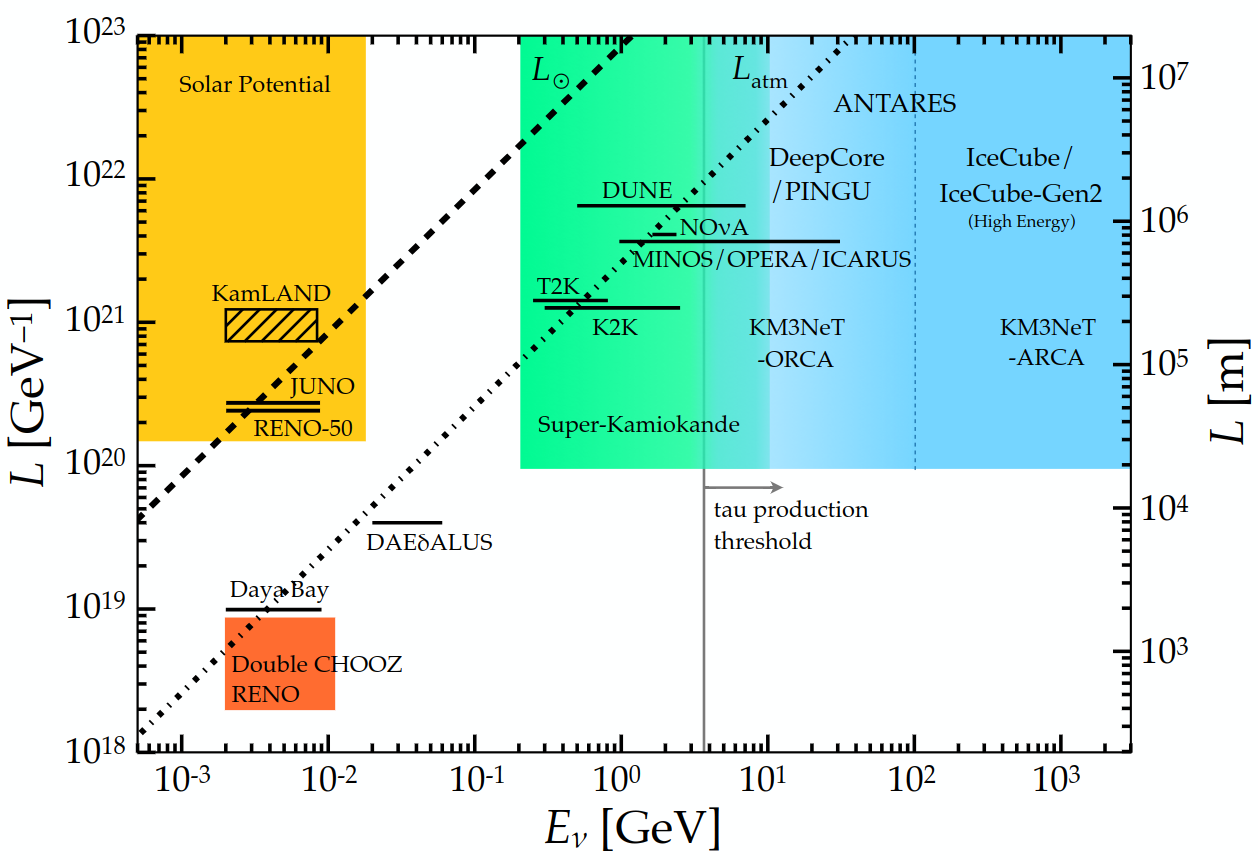
\includegraphics[width=0.7\textwidth, trim={0mm 0mm 0mm 0mm}, clip,page=1]{figures/theory/le_experiments}
	\caption{Neutrino oscillation experiments in baseline $L$ and energy $E$. Figure from \cite{ic_neutrino_2018}.}
	\label{fig:all_neutrino_expts}
\end{figure}

\subsection{Solar Neutrinos}
Solar neutrinos emanate from various nuclear fusion products and decays in the sun. \autoref{tab:solar_flux} shows the fluxes for various sources, where the $pp$ flux is strongest. However, the neutrino energy is often below threshold for the largest contributors to the flux, and most solar neutrino experiments measure the $^{8}\text{B}$ flux, shown in \autoref{fig:solar_flux}.
\begin{table}[h]
	\begin{tabular}{l | c c}
		\hline
		\hline
		Reaction & Label & Flux ($\text{cm}^{-2} \text{s}^{-1}$) \\
		\hline
		$p+p\rightarrow ^{2}\text{H} + e^+ + \nu_e$ & $pp$ & $5.95\times10^{10}$ \\
		$p+e^-+p\rightarrow ^{2}\text{H} \nu_e$ & $pep$ & $1.40\times10^{8}$ \\
		$^{3}\text{He} + p\rightarrow ^{4}\text{H} + e^+ + \nu_e$ & $hep$ & $9.3\times10^{3}$ \\
		$^{7}\text{Be} + e^- \rightarrow ^{7}\text{Li} + \nu_e$ & $^{7}\text{Be}$ & $4.77\times10^{9}$ \\
		$^{8}\text{B} \rightarrow ^{8}\text{Be}* + e^+ \nu_e$ & $^{8}\text{B}$ & $5.05\times10^{6}$ \\
		\hline
		\hline
	\end{tabular}
	\caption{Integrated solar neutrino flux from various solar processes in the $pp$ chain. Table replicated from \cite{solar_review}.}
	\label{tab:solar_flux}
\end{table}

\begin{figure}[h]
	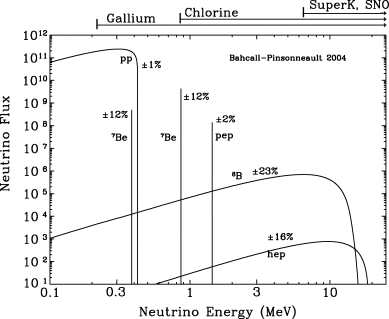
\includegraphics[width=0.5\textwidth, trim={0mm 0mm 0mm 0mm}, clip,page=1]{figures/theory/solar_flux}
	\caption{Solar flux from different $pp$ chain fusion sources, including thresholds of experiments. Figure from \cite{sno_solar_flux}.}
	\label{fig:solar_flux}
\end{figure}

R. Davis and J. Bachall continued their 1964 measurements\cite{davis} of the solar neutrinos from $^{8}\text{B}$ and in 1968\cite{davis_sun} announced a solar $\nu_e$ flux factor seven of the expected ($\sim2\sigma$ significance), at the time attributed to inaccurate solar model calculations. This was the birth of the ``solar neutrino problem'', which Bruno Pontecorvo and Vladimir Gribov in 1969\cite{pontecorvo_gribov} proposed solving by invoking a $\nu_e\leftrightarrow\nu_\mu$ oscillation similar to $K^0 \leftrightarrow\bar{K}^0$, giving rise to the PMNS paradigm. In 1989, the Kamiokande experiment\cite{kamiokande_solar} confirmed the result, measuring a solar neutrino flux from $^{8}\text{B}$  of $\sim0.5$ the expected, agreeing with the higher statistic data from Homestake\cite{davis_sun2}. The solar neutrino deficit was confirmed from the low threshold detectors SAGE\cite{sage_solar} and GALLEX\cite{gallex_solar}, additionally capable of detecting $p p$ neutrinos using $^{71}\text{Ga}+\nu_e \rightarrow ^{71}\text{Ge}+e^-$.

The Sudbury Neutrino Observatory (SNO) put the nail in the coffin in 2002\cite{sno_solar} by measuring the solar $\nu$ from $^{8}\text{B}$ in three channels: $\nu_e + d \rightarrow p+p+e^-$ (CC), $\nu_x + d\rightarrow p+ n + \nu_x$ (NC) and $\nu_x + e^- \rightarrow \nu_x+e^-$ (ES). The measured fluxes had a $\nu_e$ component consistent with previous measurements, a strong non-$\nu_e$ component 5.3$\sigma$ above zero, and a NC component consistent with predictions from solar models.

Additionally, the low threshold, low background, Borexino experiment detected solar neutrinos from the $^{8}\text{B}$, $^{7}\text{Be}$, $pep$, and $pp$ processes\cite{borexino_summary}. The final stages of Borexino aims to measure the CNO cycle and the next-generation SNO experiment, SNO+, aims to confirm and improve these measurements, and make detailed measurements of the MSW effect, solar metallicty and luminosity.

Although the solar neutrino oscillation parameters $\Delta m^2_{21}$ and $\theta_{21}$ are considered well-constrained, there is $\sim 2\sigma$ tension on $\Delta m^2_{21}$ between measurements at SK and SNO (which are compatible), and the long baseline reactor anti-electron-neutrino experiment, KamLAND\cite{m2_tension}, mentioned later.

\subsection{Atmospheric Neutrinos}
Atmospheric neutrinos are emitted when cosmic rays interact with nuclei in the earth's atmosphere, producing mesons which decay into neutrinos, amongst other particles. The primary decay is the pion decay,
\begin{gather*}
	\pi^\pm \rightarrow \mu^\pm + \nu_\mu(\bar{\nu}_\mu) \\
	\mu^\pm \rightarrow e^\pm + \bar{\nu}_\mu (\nu_\mu) + \nu_e (\bar{\nu}_e)
\end{gather*}
giving rise to a total of three neutrinos. The neutrino flux from Honda\cite{honda_flux} is shown in \autoref{fig:atmos_flux}, which peaks in the 1-100 GeV region, notably higher than the solar neutrinos.
\begin{figure}[h]
	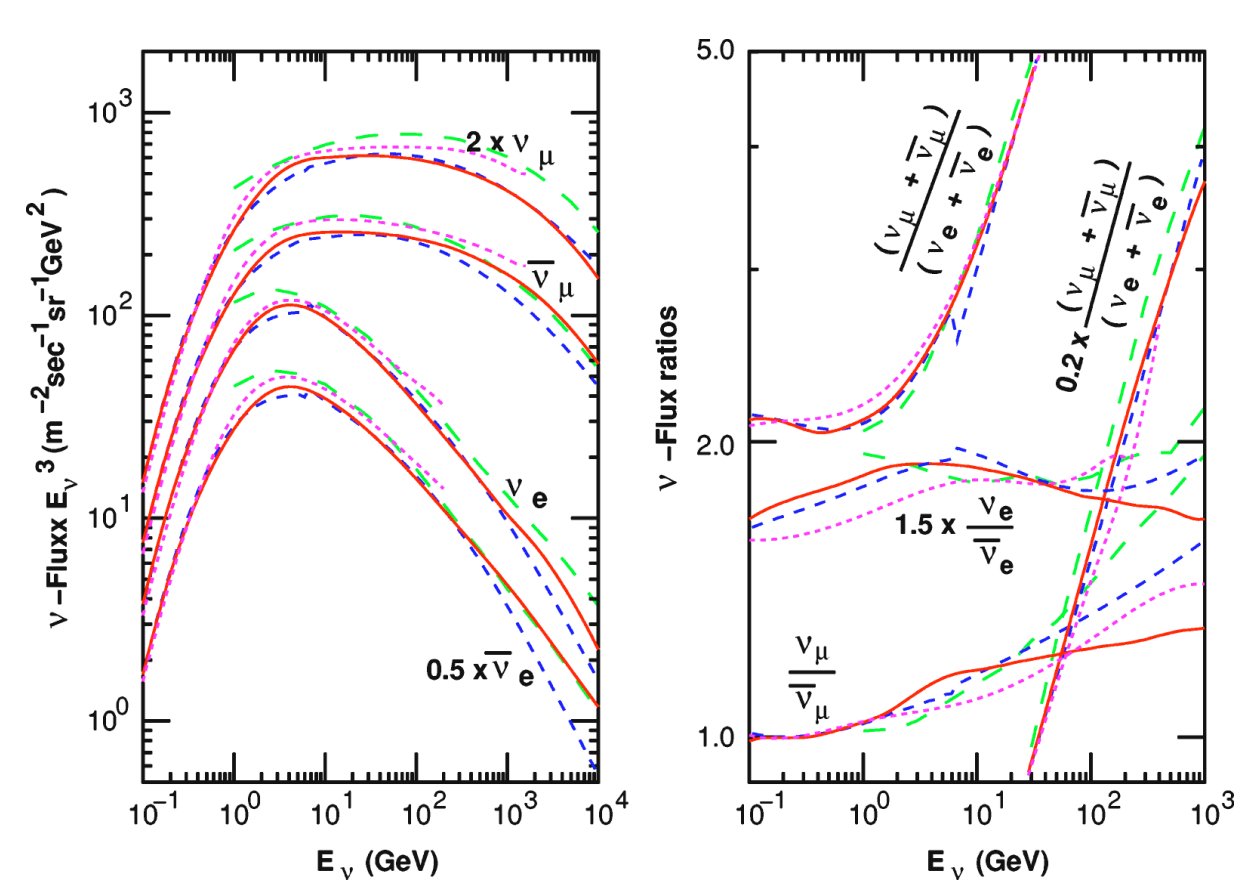
\includegraphics[width=0.7\textwidth, trim={0mm 0mm 0mm 0mm}, clip,page=1]{figures/theory/honda_flux}
	\caption{Atmospheric neutrino flux from \cite{honda_flux}.}
	\label{fig:atmos_flux}
\end{figure}

In 1965 F. Reines\cite{reines_atmos} and C.V. Achar\cite{india_atmos_hint} first saw hints of atmospheric $\nu_\mu$ appearance in deep underground laboratories through $\nu_\mu(\bar{\nu}_\mu) + X \rightarrow \mu^\pm + X'$. The Irvine-Michigan-Brookhaven (IMB) experiment observed deficits of $\nu_\mu$ interactions in 1986\cite{imb}, and Kamiokande II in 1988\cite{kamiokande_atmos_hint} verified this and found muon-like events of $59\pm7\%$ the prediction, although good agreement of electron-like single-prong events. The Soudan-2 experiment\cite{soudan2} also saw indications of muon neutrino deficiency with a flavour ratio of $0.72\pm0.19^{+0.05}_{-0.07}$ relative expectation. 

When SK in 1998 published\cite{sk_disc} their high-statistics\footnote{4353 fully-contained and 301 partially-contained events} $\nu_\mu$ data, they found $R=\left( \mu/e \right)_\text{Data}/\left( \mu/e \right)_\text{MC} =0.65\pm0.05\pm0.08$. They additionally fitted the oscillation parameters, finding the data was well described by $\nu_\mu \leftrightarrow \nu_\tau$ rather than $\nu_\mu \leftrightarrow \nu_e$. The summary of flavour ratios for atmospheric neutrino is seen in \autoref{fig:atmos_ratio}, where the majority of the high precision data sits at $R=0.5-0.8$.
\begin{figure}[h]
	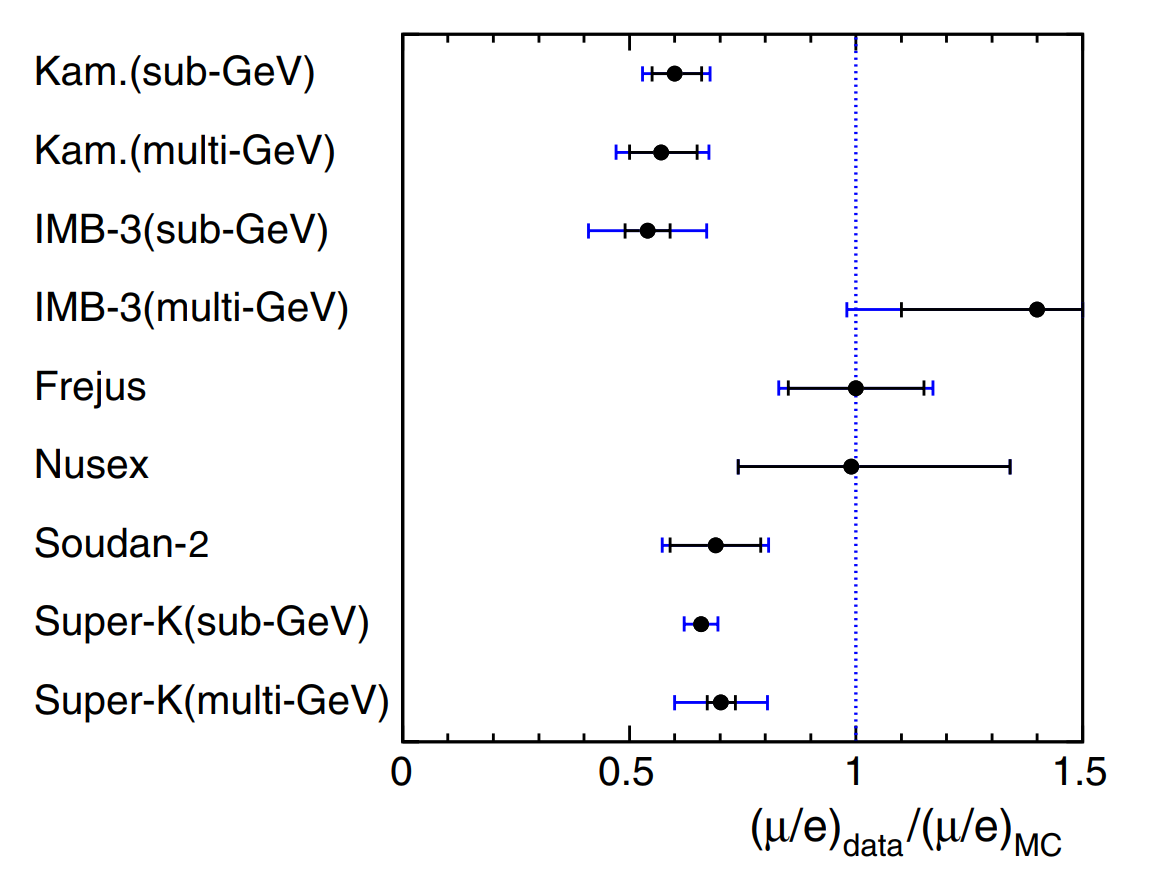
\includegraphics[width=0.7\textwidth, trim={0mm 0mm 0mm 0mm}, clip,page=1]{figures/theory/flavour_ratio}
	\caption{Measured flavour ratios for various atmospheric neutrino experiments. Figure from \cite{kajita_summary}.}
	\label{fig:atmos_ratio}
\end{figure}

Atmospheric neutrino observatories after the mid 2000s have focussed on measuring $\nu_\mu\rightarrow\nu_\mu$ to increasing precision. Furthermore, by isolating regions of specific zenith angle (and so baseline $L$), the extent of the matter effects are also studied, which may resolve the ordering of the mass states. This is largely the focus of IceCube\cite{icecube}, ANTARES\cite{antares}, SNO+ and SK's atmospheric neutrino programme. SK has also made attempts at isolating $\nu_\tau$ events\cite{superk_tau}, claiming $4.6\sigma$ discovery of $\nu_\tau$ appearance in 2017. A summary of some recent results including complementary long baseline accelerator neutrino experiments can be seen in \autoref{fig:atmos_data}.
\begin{figure}[h]
	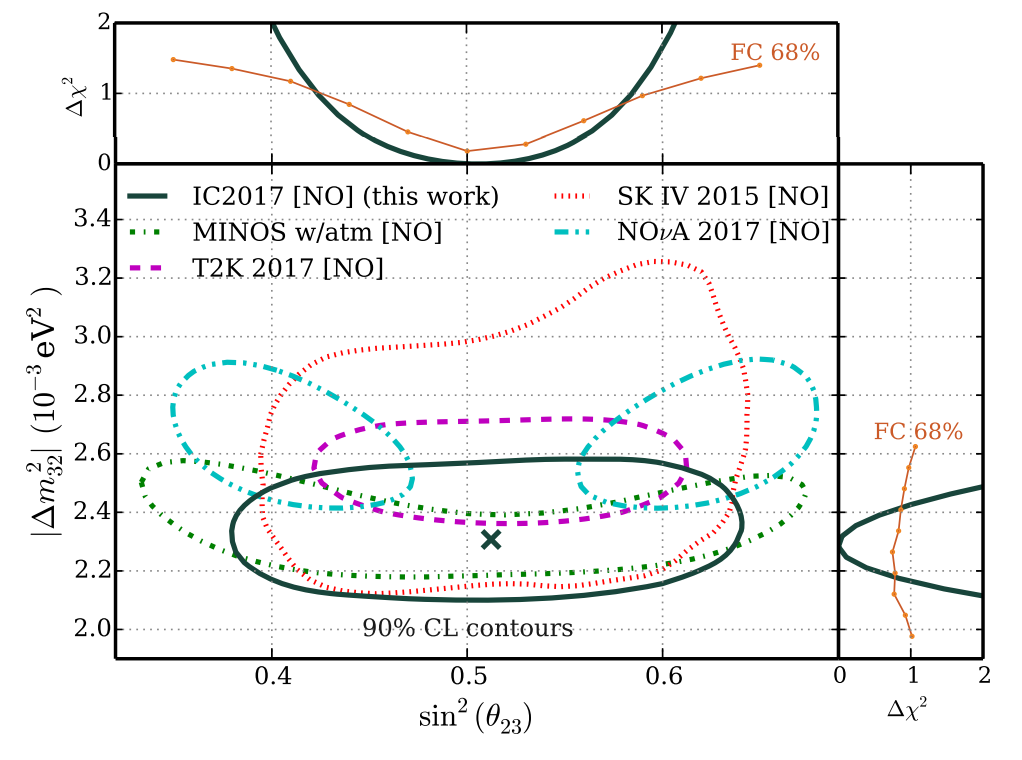
\includegraphics[width=0.7\textwidth, trim={0mm 0mm 0mm 0mm}, clip,page=1]{figures/theory/icecube_comp}
	\caption{Measured atmospheric oscillation parameters from recent atmospheric and long baseline accelerator neutrino experiments, assuming normal ordering. Figure from \cite{icecube}.}
	\label{fig:atmos_data}
\end{figure}

\subsection{Accelerator Neutrinos}
Accelerator neutrinos are similar to atmospheric neutrinos in energy, baseline and production mechanism. The neutrinos are made by impinging protons from accelerators on targets, producing a flurry of mesons which decay into neutrinos, amongst others. Experiments often have the ability to deflect and/or focus mesons after the target, enabling sign and thus $\nu_\mu$ vs $\bar{\nu}_\mu$ selection. In contrast to atmospheric neutrinos, accelerator neutrinos are primarily ($\sim90\%$) muon flavoured.

The driver behind the accelerator programme was the atmospheric neutrino oscillations outlined above. Since the neutrino energy and baseline are tuned and chosen for an accelerator experiment, the oscillation dip can be bombarded with statistics. Furthermore, the dependence on the atmospheric flux simulation is removed\cite{lbnl_review}. The disadvantage is the reduced total flux at the far-detector, generally forcing the baseline to $L<1000\text{ km}$ which limits the impact of the matter effect and sensitivity to the mass ordering. The majority of long baseline accelerator neutrino experiments include a near detector which samples the beam before any long baseline oscillations have taken place.

The short-baseline ($L\sim 1\text{ km}$) accelerator neutrino experiments, such as MiniBooNE\cite{mb_design}, MINER$\nu$A\cite{minerva_design}, and the upcoming SBND programme\cite{sbnd}, are generally intended to measure neutrino cross-sections and perform short baseline oscillation searches. They may also serve as neutrino beam monitors for other experiments. The interaction measurements are used to inform neutrino event generators\cite{neut,genie,NuWro}, aiding in reducing systematic uncertainties for neutrino cross-section and oscillation experiments.

The pioneering long-baseline ($L\sim 100-1000\text{ km}$) experiments MINOS\cite{minos_obs} and K2K\cite{k2k_obs} confirmed the atmospheric neutrino mixing in $\nu_\mu \rightarrow \nu_\mu$, finding compatible oscillation parameters. The searches for $\nu_\mu \rightarrow \nu_e$ were not statistically significant\cite{k2k_noobs,minos_disc}, and were discovered by the next generation experiments T2K\cite{t2k_disc} and NO$\nu$A\cite{nova_disc}, with the $\bar{\nu}_\mu \rightarrow \bar{\nu}_e$ oscillation hinted at by NO$\nu$A at Neutrino 2018\cite{nova_neutrino2018}. The Japanese experiments K2K and T2K have consistently used the 50,000 tonne water Cherenkov detector SK\cite{superk} as their far detector, with plastic scintillator based near-detectors and a baseline of $L\sim250\text{ km}$ and $E\sim0.5-2\text{ GeV}$. Both MINOS and NO$\nu$A use(d) purpose-built matching near and far-detectors, allowing for many detector systematics to be reduced, with $L\sim700\text{ km}$ and $E\sim2-5\text{ GeV}$.

In Europe, the OPERA\cite{opera} experiment was designed to look for the dominant $\nu_\mu \rightarrow \nu_\tau$ oscillation at $L\sim700\text{ km}$. The ICARUS\cite{icarus} experiment searched for $\nu_\mu\rightarrow\nu_e$ from steriles observed by LSND\cite{lsnd} and MiniBooNE\cite{miniboone_sterile}, which have been questioned in the community\cite{lsnd_refute}. The detection threshold for the charged current interaction $\nu_\tau + X \rightarrow \tau + X'$ is $E_\nu\sim 3.5\text{ GeV}$, so the neutrino beam from CERN to Gran Sasso (CNGS)\cite{cngs} was wide-band with $E_\nu = 10-25\text{ GeV}$. The $\tau$ detection requires very fine granularity and OPERA used nuclear emulsions whereas ICARUS pioneered the use of liquid argon TPCs in neutrino physics. OPERA claimed $\nu_\tau$ appearance\cite{opera_final_tau} at 6.1$\sigma$, and both OPERA and ICARUS found no evidence of sterile neutrinos\cite{icarus_lsnd,opera_lsnd}.

\subsection{Reactor Anti-Neutrinos}
Reactor neutrinos are formed in $\beta$ decay of fission products in nuclear reactors, e.g. $^{231}\text{Th} \rightarrow ^{231}\text{Pa} + e^- + \bar{\nu}_e$ and $^{215}\text{Po} \rightarrow ^{211}\text{Pb} + e^- + \bar{\nu}_e$. The neutrino flux depends on the relative fission yields of the products, but generally have a similar energy to solar neutrinos, in the 1-10 MeV range. A test reactor flux is shown for reference in \autoref{fig:reactor_flux}.
\begin{figure}[h]
	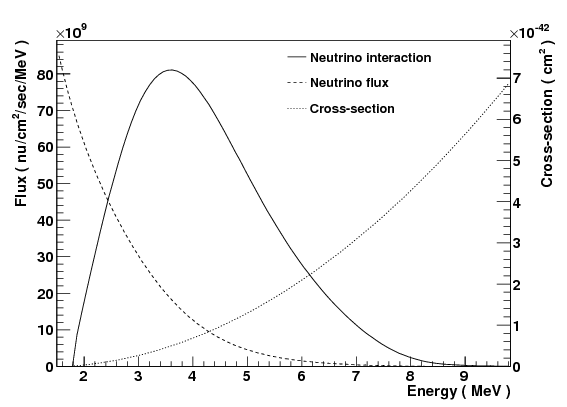
\includegraphics[width=0.6\textwidth, trim={0mm 0mm 0mm 0mm}, clip,page=1]{figures/theory/reactor_flux}
	\caption{Reactor flux for the Japanese experimental fast reactor, JOYO. Figure from \cite{reactor_flux}.}
	\label{fig:reactor_flux}
\end{figure}

They are exclusively detected by the IBD interaction, in which the $e^+ + e^- \rightarrow 2\gamma$ are measured in scintillator. Many experiments additionally dope or surround the scintillator with a high neutron capture element (e.g. $^{6}\text{Li}$ or $^{157}\text{Gd}$). In the case of Gd doping, the signal consists of the prompt $2\gamma$ followed by a $\sim30\mu\text{s}$ delayed $\gamma$ cascade with $E_\gamma^{tot}\sim8\text{ MeV}$ from the Gd de-excitation, facilitating signal-background separation. 

Similarly to accelerator neutrinos, the reactors can be split by baseline. Short baseline experiments with $L\sim1-2\text{ km}$ perform world-leading measurements of $\Delta m^2_{13}$ and $\sin^2\theta_{13}$, and probing parts of the sterile neutrino spectrum. Daya Bay\cite{daya_bay_disc}, RENO\cite{reno_disc} and Double Chooz\cite{double_chooz} all measured a relatively large $\sin^2 \theta_{13}$, enabling $\nu_e$ appearance to be found at long baseline neutrino experiments such as T2K and NO$\nu$A. The short baseline reactor results on $\sin^2\theta_{13}$ are often used in atmospheric and accelerator oscillation analyses for increased sensitivity to the 2,3 parameters and $\delta_{CP}$. A summary plot of the measured parameters by short baseline reactor and long baseline accelerator neutrino oscillation experiments is shown in \autoref{fig:13_sector}.
\begin{figure}[h]
	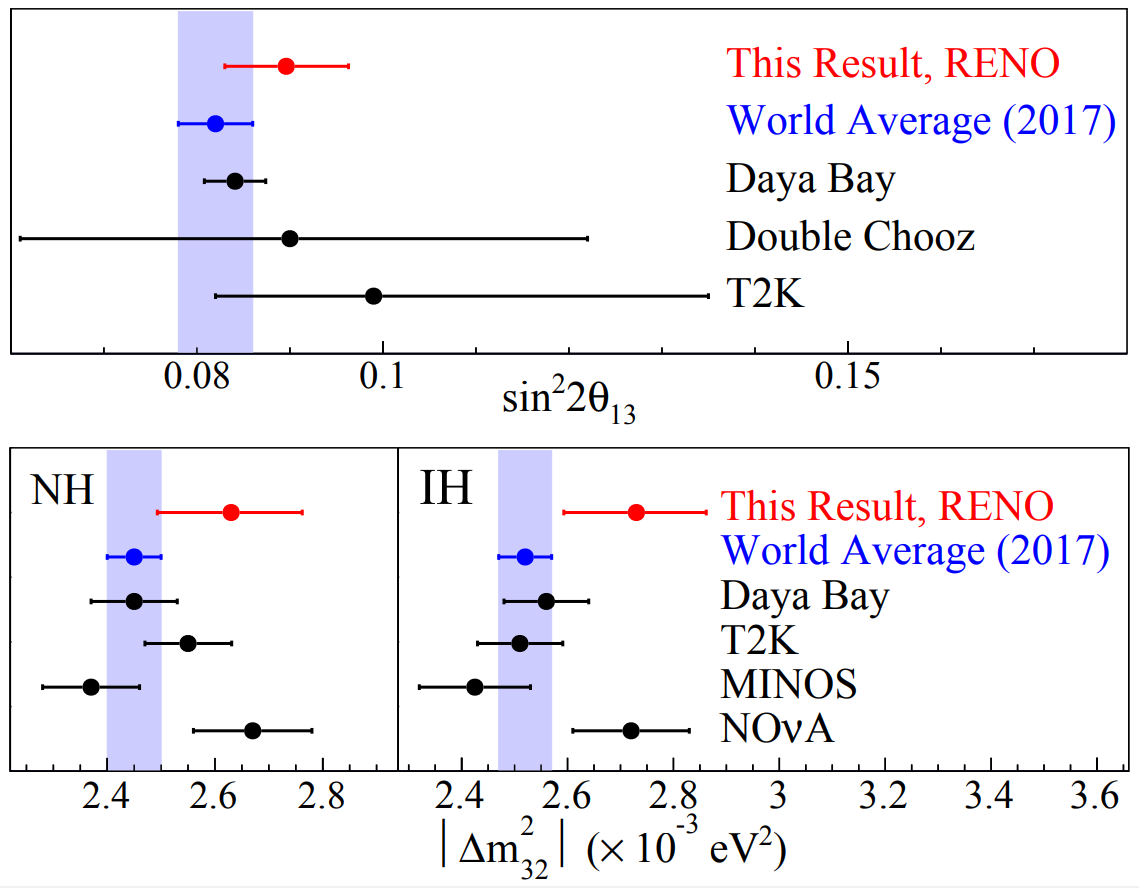
\includegraphics[width=0.5\textwidth, trim={0mm 0mm 0mm 0mm}, clip,page=1]{figures/theory/reno_theta_dm13}
	\caption{$\Delta m^2_{23}$ and $\sin^2 2\theta_{13}$ measurements from reactor (Daya Bay\cite{daya_bay}, RENO\cite{reno_new} and Double Chooz\cite{double_chooz_old}) and accelerator (T2K\cite{t2k_2015}, NO$\nu$A\cite{nova_2017} and MINOS\cite{minos_numu_nue}) neutrinos. Figure from \cite{reno_new}.}
	\label{fig:13_sector}
\end{figure}

The only medium baseline experiment ($L\sim50\text{ km}$) under construction is JUNO\cite{juno}. The RENO collaboration has proposed\cite{reno_50} building a far detector site for RENO, equivalent to JUNO, although groundbreaking has not yet commenced. The medium baseline aims to measure the neutrino mass ordering by separating the oscillations into fast and slow parts from $\Delta m^2_{23}$ and $\Delta m^2_{12}$, and improve measurements of $\sin^2 \theta_{12}$.

KamLAND is the only long baseline ($L\sim180\text{ km}$) reactor anti-neutrino experiment. It measured $\bar{\nu}_e$s from 56 Japanese nuclear power reactors with good sensitivity to $\Delta m^2_{21}$. Additionally, combining KamLAND with SNO and SK solar data reduces uncertainties on $\Delta m^2_{21}$ and $\tan^2\theta_{12}$, as shown in \autoref{fig:21_sector}. These results are used as priors in the T2K oscillation analyses.
\begin{figure}[h]
	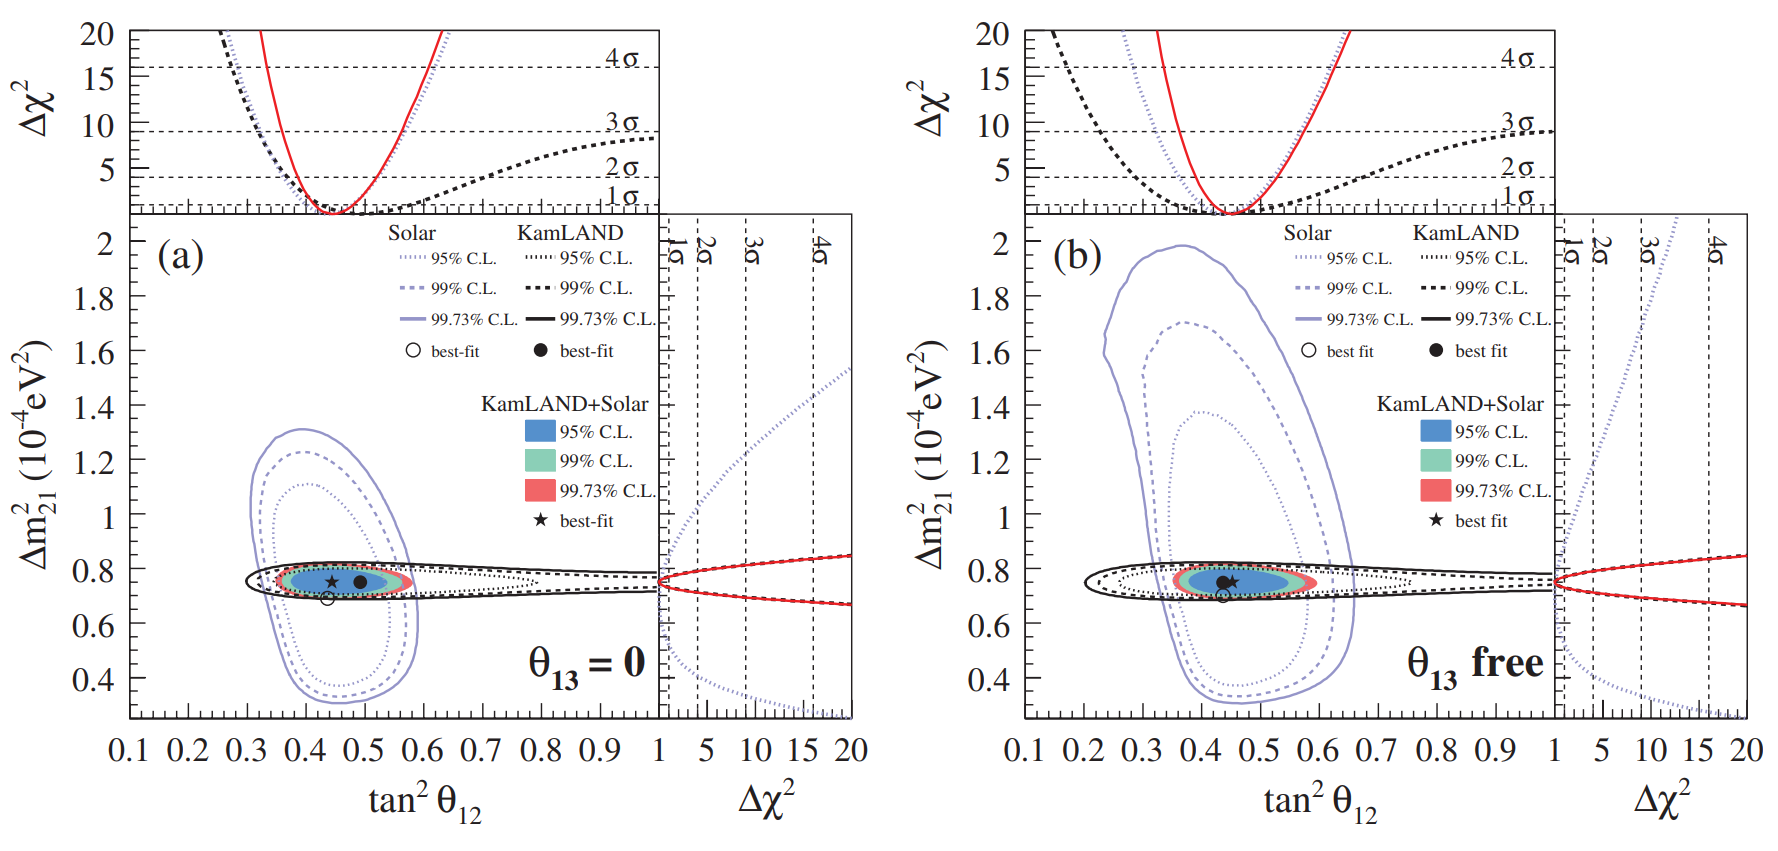
\includegraphics[width=0.7\textwidth, trim={0mm 0mm 0mm 0mm}, clip,page=1]{figures/theory/kamland_solar_comb}
	\caption{$\Delta m^2_{21}$ and $\theta_{21}$ measurements from KamLAND, SNO and SK (Solar). Figure from \cite{kamland_2011}.}
	\label{fig:21_sector}
\end{figure}

The short baseline reactors at $\sim1\text{ km}$ have measured neutrino excess at $E_\nu\sim5\text{ MeV}$\cite{double_chooz, daya_bay, reno}, which is currently unresolved. The culprit is claimed to be either poor neutrino flux modelling or a sterile neutrino\cite{huber_neos,steriles}. As a result, very short baseline ($L\sim10-20\text{ m}$) experiments NEOS\cite{neos}, DANSS\cite{danss}, PROSPECT\cite{prospect}, STEREO\cite{stereo} and SoLi$\delta$\cite{solid} have looked for $\bar{\nu}_e$ disappearance and have not found evidence of a sterile signal and confirmed hints of a 5 MeV excess.